% emphasize the special characteristic of hardware-related software
\section{Problem in Managing HW/SW Interface Traceability Links}
\label{sec:problem}

An interface between hardware and software is typically composed of registers exposed by hardware devices and accessible by software. The implementation of the interface should conform to the specification in order to function correctly. Suppose we have to maintain and understand this implementation, we need to establish the relationships between the implementation and the specification.
\begin{figure}[h!]
  \begin{center}
    \begin{tabular}{c}
\begin{minipage}[b]{\linewidth}
  \centering
  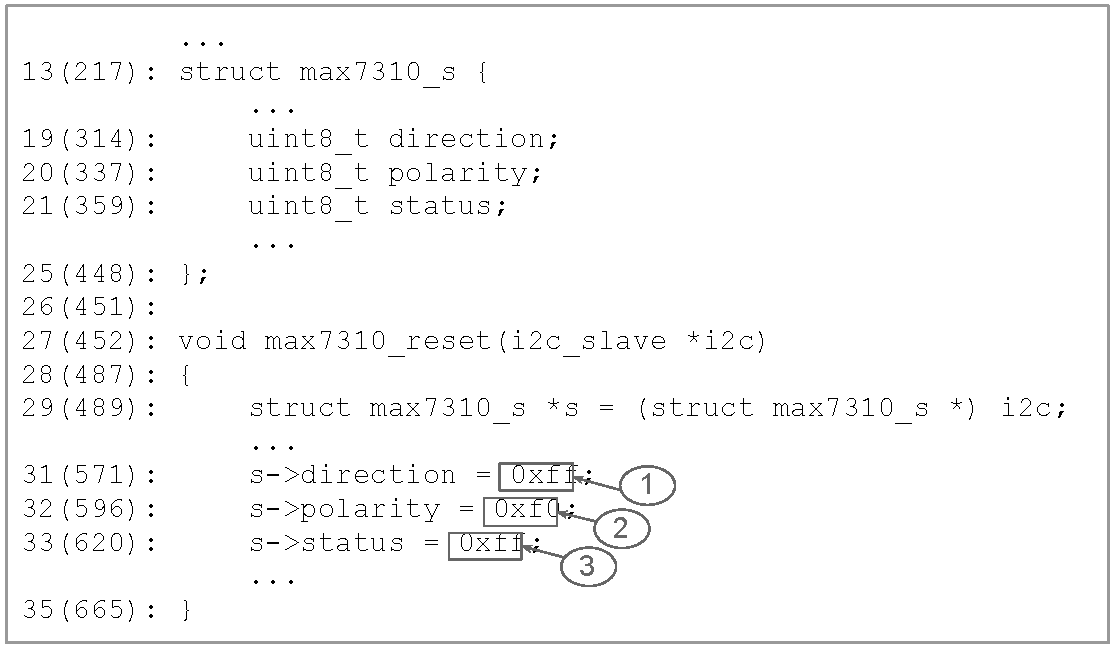
\includegraphics[width=0.8\linewidth]{code1}
\end{minipage}\\
(a) Older Version\\
\\
\begin{minipage}[b]{\linewidth}
  \centering
  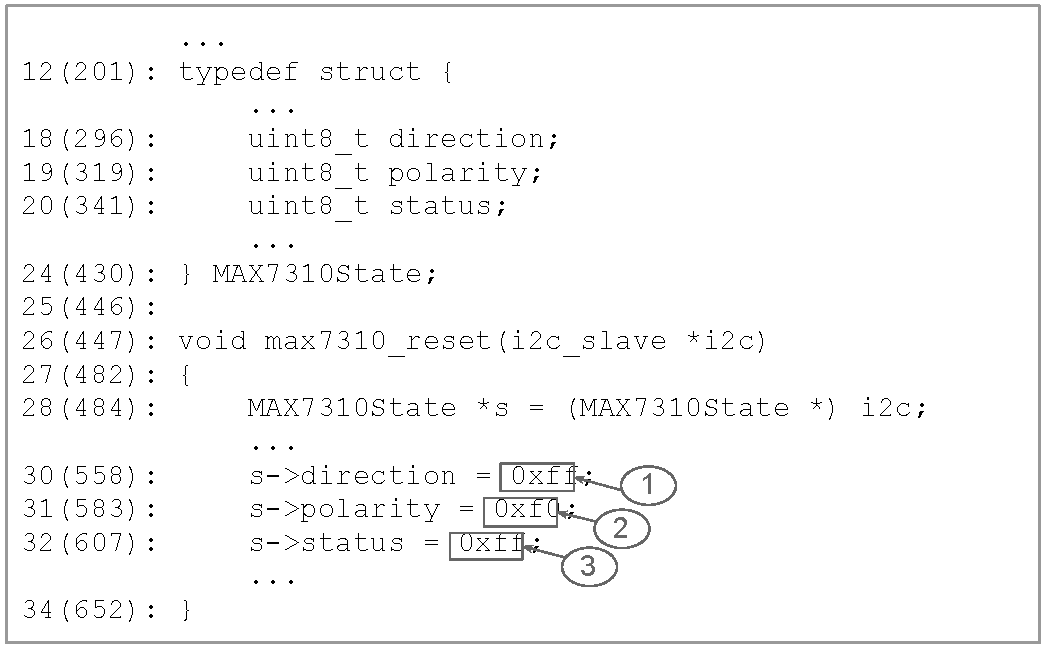
\includegraphics[width=0.8\linewidth]{code2}
\end{minipage}\\
(b) Newer Version
\end{tabular}
  \caption{ Corresponding code snippets from two versions of the MAX7310 virtual device from the QEMU virtual machine. This code defines a function to reset the device.}
  %However, it is unclear why the registers are reset to the values labeled 1, 2 and 3. To know the answer, one has to refer to the specification.}
\label{fig:code}
\end{center}
\end{figure}
Figure~\ref{fig:code}(a) presents part of code extracted from the MAX7310 virtual device from QEMU. A virtual device is a software implementation emulating a hardware device. MAX7310 is a 8-bit I/O port expander. QEMU (Quick EMUlator)~\cite{Bellard05} is a virtual machine widely used in industry to assist hardware-related software development. The source code for this implementation is written in the C language. From the name of the function, we can guess it is trying to reset the device to its initial state. However, we cannot figure out what the values in the right sides of the assignment statements mean only by reading the code here. Figure~\ref{fig:spec} includes the information extracted from the specification of MAX7310. In this figure, we can see three tables for three registers: polarity register, direction register, and status register. These tables present the bit arrangement and the default value for each register. We can see that the values used in the code are defined in the specification. The code uses the hex format, and the specification uses the binary format. The piece of code and the piece of specification labeled with the same number are related, which means the piece of specification explains the piece of code with the same label.

\begin{figure}
  \centering
  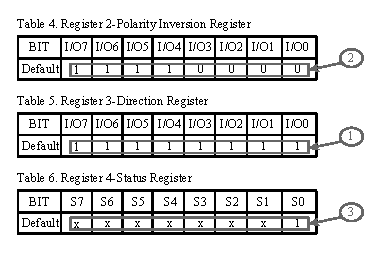
\includegraphics[width=0.7\textwidth]{spec}
  \caption{Specification Example. This is part of the MAX7310 specification, including three tables which define default values for three registers.}
  \label{fig:spec}
\end{figure}

% in the directory including max7310.c: git log --follow --all -p max7310.c > a.txt
Implementation code evolves all the time in its lifecycle. By checking the QEMU repository, we found that the first version of the code in Figure~\ref{fig:code} was created on May 23, 2007, and the last change was on May 1, 2013. This code has changed 21 times till now, and it still keeps changing.
Figure~\ref{fig:code}(b) shows a newer version of the code in Figure~\ref{fig:code}(a). Line 13, 25 and 29 of the code in Figure~\ref{fig:code}(a) has changed to the line 12, 24 and 28 in Figure~\ref{fig:code}(b). Compared to code, specification is often relatively stable. The specification in Figure~\ref{fig:spec} only has three versions, and the last change happened in 2005. The specification remains unchanged since the code was created.

This example, although simple, reveals three basic requirements for managing traceability links between specification and implementations as follows.

\smallskip
\noindent 
\textbf{Requirement 1:} Traceability links should be able to uniquely identify and accurately locate relevant pieces of code in the source file and pieces of specification in the specification file. As in the example, there should be a simple and unique way to locate the code pieces and specification pieces surrounded by the boxes labeled by 1, 2 and 3.

\smallskip
\noindent
\textbf{Requirement 2:} Traceability links should be able to provide references on the statement level or expression level for source code and at the sentence level or word level for specification. As in this example, the code pieces and specification pieces surrounded by the boxes labeled by 1, 2 and 3 are all on the expression level and the word level.

\smallskip
\noindent
\textbf{Requirement 3:} Traceability links should be immune from the evolution of unrelated code. We need to ensure that an identifier created for the old version of code works for the new version if the code piece referred to by the identifier does not change.

